

%\documentclass[pdf,gyom,slideColor,colorBG,nototal]{prosper}

\documentclass[blue,notes=noshow,slidestop,compress]{beamer}  %% mit
                                %% handout-option: die
                                %% overlays sind auf
                                %% einen schlag
                                %% notes=show

%\newif\ifweb\webtrue
\def\version{5}
\def\status{transient}
\def\docdate{17.~01.~2005}




%%%%%%%%%%%%%%%%%%%%%%%%%%%%%%%%%%%%%%%%%%%%%%%%%%%%%%%%%%%%%%%
%% $Id$ %%
%%%%%%%%%%%%%%%%%%%%%%%%%%%%%%%%%%%%%%%%%%%%%%%%%%%%%%%%%%%%%%%
%%% Local Variables: 
%%% mode: latex
%%% TeX-master: "main"
%%% End: 


\usepackage{hevea}
\usepackage{hyperref}
%\usepackage{url}
\usepackage[english]{babel}
\usepackage{epsfig}
\usepackage{tfheader}
\usepackage{a4wide}
\usepackage[latin1]{inputenc}

\usepackage{graphicx}
\graphicspath{{../figures/}} %% cool!

\usepackage{psfrag}

\ifweb

\htmlfoot{\hrulefill{}
  {\footnotesize Pages last (re-)generated \today}}
\renewcommand{\@bodyargs}{bgcolor="white" alink="red" vlink="\#407999"  link="\#7070ff"}  
\fi







%%% Local Variables: 
%%% mode: latex
%%% TeX-master: "main"
%%% End: 

%% common macro files for the projects


\newcommand{\NONAME}{Somename}


\newcommand{\Coma}{\textsl{Coma}}

\newcommand{\cvs}{cvs}
\newcommand{\Java}{\textsc{Java}}
\newcommand{\Cplusplus}{C$^{++}$}
\newcommand{\javadoc}{\textsc{javadoc}}



\newcommand{\team}[1]{\textbf{Responsible:} #1\bigskip{}}


\newcommand{\bnfdef}               {::=}
\newcommand{\bnfbar}               {\mathrel{|}}

\newcommand{\suchthat}{\mathrel{\mid}}
\newcommand{\union}  {\cup}
\newcommand{\intersect}  {\cap}
\newcommand{\sizeof}[1]  {{\mid}{#1}{\mid}}
\newcommand{\sem}    [2]        {[\![#2]\!]_{#1}}      %semantics

\newenvironment{diagram}{\begin{displaymath}}{\end{displaymath}}


%%% Local Variables: 
%%% mode: latex
%%% TeX-master: t
%%% End: 

%\input{macros-local}
%\input{title}

\title[Coma]{Coma (v.1)}

\author[G. Schaefer \and M. Kyas \and M. Steffen]{%
  \tiny
  {Gunnar Schaefer \and  Marcel Kyas \and Martin Steffen}}

\institute{\tiny Christian-Albrechts University  Kiel}
\titlegraphic{
  \begin{center}
    \pgfuseimage{christiane}
  \end{center}}

\date[WS 2004/05]{{\tiny Wintersemester 2004/05}}




% use option  pdf  instead of ps when not printing


\begin{document}
\maketitle

%----------------------------------------------------------------------


\section{Introduction}

\frame{\frametitle{Introduction}
  \begin{itemize}
  \item simulation of ``real'' project
  \item including all (or many) phases:
    \begin{itemize}
    \item specification
    \item realization, architecture
    \item testing, shipping
    \end{itemize}
  \item product:
  \item[]
    \shadowbox{\important{conference manager tool}: \importantxx{\Coma}} (more
  details later)
  \end{itemize}
}


\frame{\frametitle{Side conditions}
  \begin{itemize}
  \item firm \important{deadline}: end of semester!
  \item \important{heterogeneous} team
  \item unlike previous semester: almost ``theoryless'' project (in some sense)
  \item[$\Rightarrow$] one main problem will be:
    \important{cooperation}/\important{coordination}/\important{putting things together}
  \item there is no ``\important{solution}'', the solution is: what we make of
    it
  \item motives:
    \begin{itemize}
    \item ``\importantxx{Schein}'' (of course)
    \item learning to do project work/team work
    \end{itemize}
  \item roles of \importantx{supervisors:}
    \begin{itemize}
    \item \important{managers:} we are responsible for official things,
      grading, etc.
    \item \important{client:} we provide the informal spec
    \item \important{moderators} of the discussions
    \item providing \important{framework} (installing/helping to install
      software, getting literature etc), discussion partner, 
    \item technical assistance and support
    \end{itemize}
  \end{itemize}
}




\frame{\frametitle{Consequences}
  \begin{itemize}
  \item tight schedule: one semester is \important{short}
    \begin{itemize}
    \item don't \important{postpone} things
    \item be \important{open}
      \begin{itemize}
      \item tell the team: if you get delayed for some reason
      \item  better change plans than stick to unrealistic ones
      \item ask for help/offer help to others
      \item make realistic timeplans/estimations\footnote{a typical
          unrealistic (and often heared) estimation is: ``last 4 weeks my
          group only achieved  10\% of the plan, but the next two weeks
          we do 500\%.}
      \end{itemize}
    \end{itemize}
  \item<2>[]\only<2>{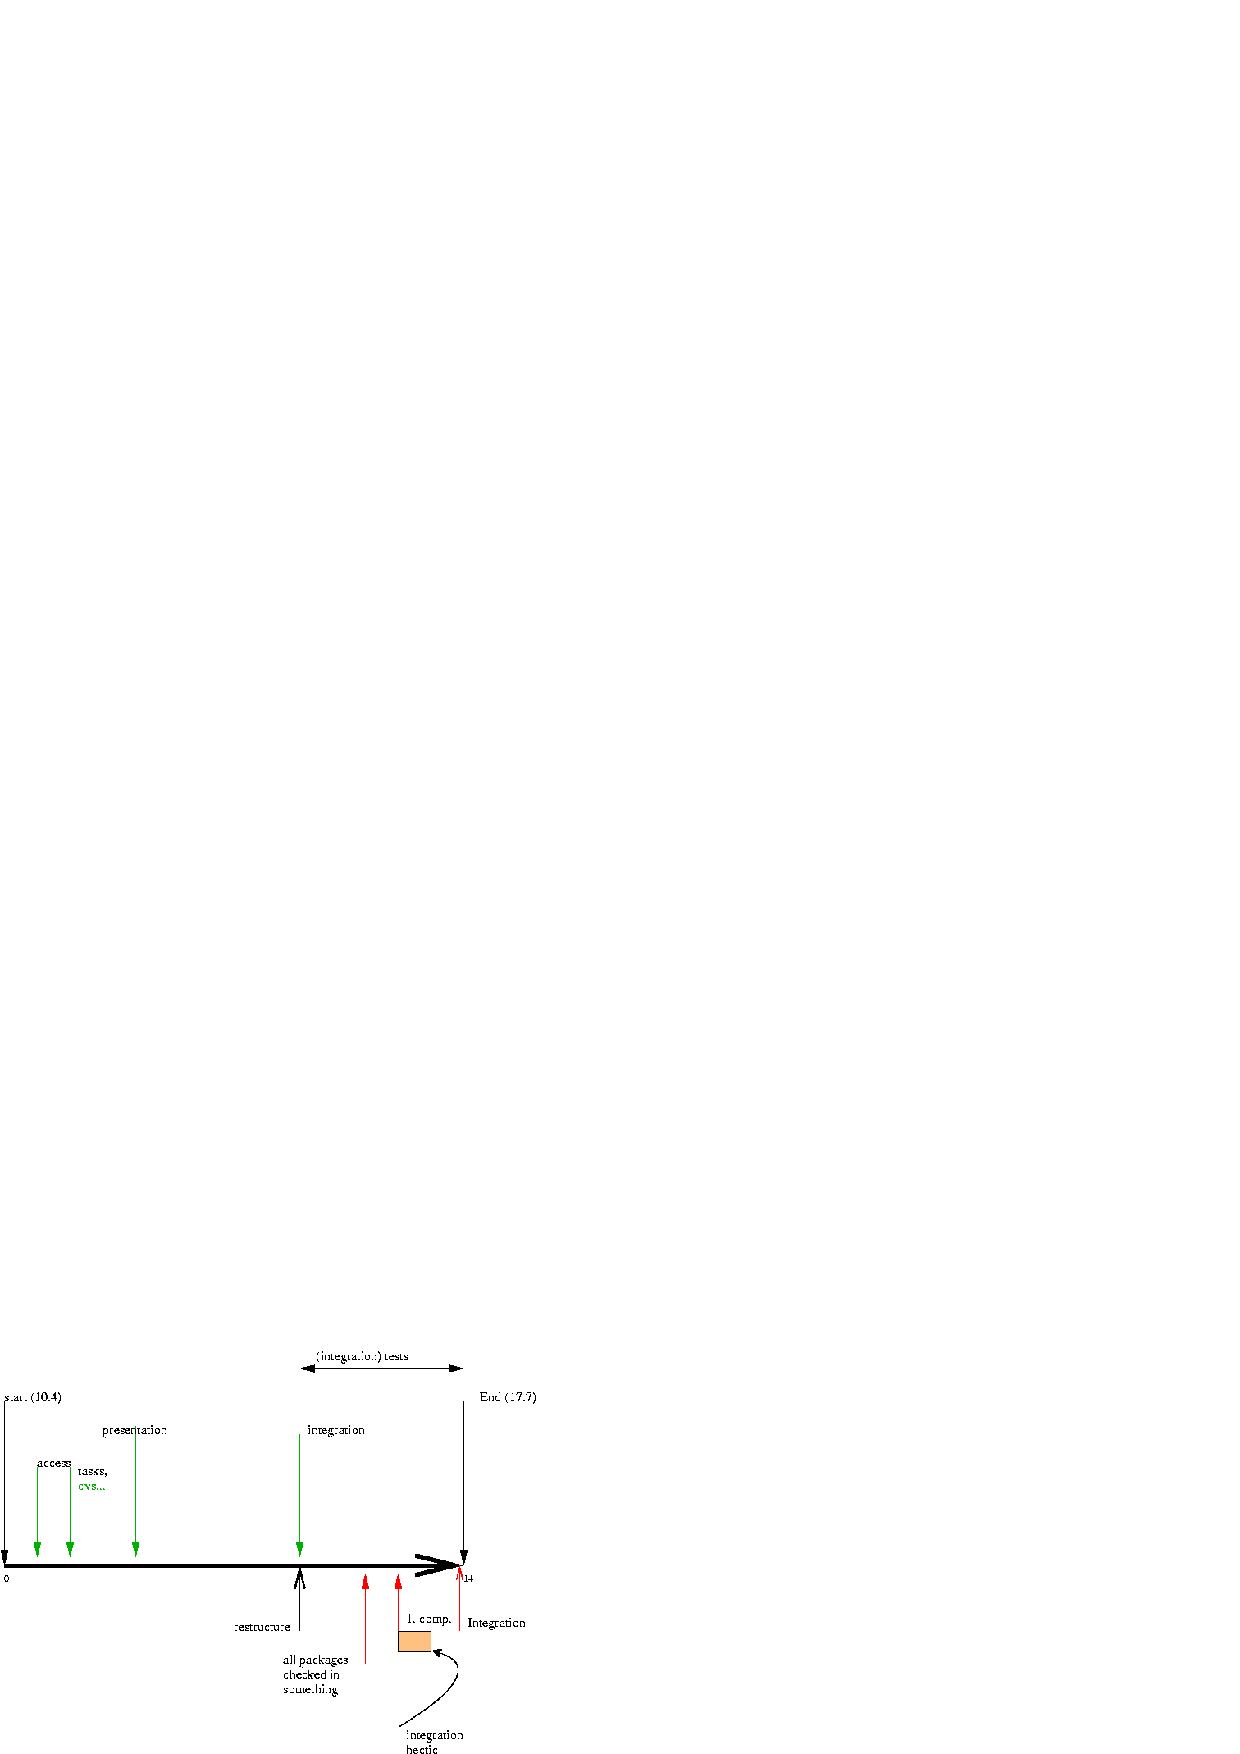
\includegraphics[clip=true,height=4.0cm]{timeline}}
  \item<3-> requirement specification is part of the task!
  \item<3-> success by
    \begin{itemize}
    \item<3-> initiative\footnote{Don't wait till someone else tells you what to
        do. Don't wait till the lazy group 12 does something.}
    \item<3-> openness, communication
    \item<4> (yes: and of course \importantxx{work} \ldots)
    \end{itemize}
  \end{itemize}
}


\frame{\frametitle{What we expect}
  \begin{itemize}
  \item active participation in \important{all} phases, in particular also
    the specification/setup phase
  \item active participation in the weekly meetings\footnote{take both parts
      \important{serious}! (the other parts, too, of course\ldots)}
  \item workable solution of the chosen task
  \item don't drop out in mid-flight
  \item timeliness
  \item during semester/end-of-semester: deliverables, demo and
    presentation(s)
  \end{itemize}
}
\section{Informal spec.}


\frame{\frametitle{\Coma}
  \begin{itemize}
  \item why this project?
  \item[$\Rightarrow$] simple reasons: 
    \begin{itemize}
    \item we (as \important{clients}) know vaguely what we ``want'',
    \item you (as \important{IT specialists}) probably don't exactly know what
      we want
    \end{itemize}
  \item conference manager:
  \item[]
    \shadowbox{
      \begin{minipage}[t]{9cm}
        A web-based tool to assist the distributed preparation,
        organi{z}ation, and processing of scientific conferences.
      \end{minipage}
    }
  \end{itemize}
}


\frame{\frametitle{Requirements}
  \begin{itemize}
  \item 4 main kinds of \important{customers}
    \begin{enumerate}
    \item  administrator: ``guru''
    \item authors: submit papers, wait for acceptance
    \item program commitee
      \begin{itemize}
      \item decides about acceptance/rejectance of contributions
      \end{itemize}
      \item chairman (1 or many): 
        \begin{itemize}
        \item boss/moderator of the program commitee
        \item taking final decision[
        \end{itemize}
    \end{enumerate}
  \item adaptability: product should be usable for many conferences
  \item ``maintainability'': product should be managable via the net
  \item ``\important{portability}'': should be deplayably/run with standard
  \item ``security'': it should not compromize the safety of the system
    software
  \end{itemize}
}

\frame{\frametitle{Possible tasks}
  \begin{itemize}
  \item data base(s)
  \item report generation, web page generation
  \item discussion tracking
  \item management of discussion status
  \item visualization of status
  \item algorithm for assignments
  \item interface for authors
  \item interface for maintainers
  \item interface for programm commitee
  \item [testing]
  \item [documentation/manual]
  \end{itemize}
}



\section{First timeline sketch}

\frame{\frametitle{Semster}
  \begin{itemize}
  \item fixed dates:
    \begin{enumerate}
    \item start: now
    \item end: end of semster: Friday, 11.\ February 2005
    \end{enumerate}
  \item[$\Rightarrow$] 15 tuesdays/ approx general 15 meeting during
    semester (i.e., without Christmas)
  \item at the end (as said)
    \begin{itemize}
    \item demo
    \end{itemize}
  \item wish: early \important{integration}\footnote{will be hard(er) this
      time.}
  \item wish: testing
  \end{itemize}
}

\frame{\frametitle{Today}
  \begin{itemize}
  \item supervisors
    \begin{itemize}
    \item introduction
    \item project intro and warm up (= now)
    \item CVS intro 
    \end{itemize}
  \item team
    \begin{itemize}
    \item personal introduction
    \item expertise of the team
    \item how many participants? 
    \item 4/8 hours?
    \item formation of \important{teams} of the \important{first phase}
    \end{itemize}
  \end{itemize}
}





\frame{\frametitle{first 2 weeks}

  \begin{itemize}
  \item get the ball rolling: $\Rightarrow$
  \item we need (at least) two teams\footnote{depending on how many we are}
    \begin{enumerate}
    \item taskforce ``\importantx{Spec}''
      \only<1>{
      \begin{itemize}
      \item explicit requirement definition of the requirement spec
      \item taking into consideration
        \begin{description}
        \item[-] manpower of the semester
        \item[-] \important{modularizability}, equal load
        \item[-] expertise of the members
        \end{description}
      \item sources
        \begin{description}
        \item[-] thinking
        \item[-] \important{discussion} with us\footnote{I.e., we need
            appointments.}
        \item[-] ``market analysis''
        \end{description}
      \item deliverables:
        \begin{description}
        \item[-] spec. document
        \item[-] presentation
        \end{description}
      \end{itemize}}
    \item taskforce ``\importantx{Tools}''
      \only<2>{
        \begin{itemize}
      \item selection of the tools/languages for the implementation
        \begin{description}
        \item[-] which database server (if any)
        \item[-] which language(s), which versions
        \item[-] \ldots
        \end{description}
      \item taking into consideration
        \begin{description}
        \item[-] manpower
        \item[-] local availability\footnote{we can of course install
            things}
        \item[-] expertise!
        \end{description}
      \item sources
        \begin{description}
        \item[-] discussion
        \item[-] ``market analysis''
        \end{description}
      \item deliverable
        \begin{description}
        \item[-] tools spec (versions)
        \item[-] presentation
        \item[-] expertise (i.e., being able to help the others)
        \item[-] availability of the tools
        \end{description}
      \end{itemize}}
  \item taskforce \importantx{Testing}
    \only<3>{
    \begin{itemize}
    \item make a test concept, deliverables: as the other task forces
    \end{itemize}}
  \end{enumerate}
\end{itemize}
}



\frame{\frametitle{Till/during next week}
  \begin{itemize}
  \item members
    \begin{itemize}
    \item get cvs \important{ready}(see handout)
    \item organize your \important{workplace}
    \item first appointments?
    \end{itemize}
  \item coordinators:
    \begin{itemize}
    \item make first informal spec ready
    \item make email adresses available
    \item finalize web-page
    \item organize further literature
    \end{itemize}
  \end{itemize}
}

\section{Misc}

\frame{\frametitle{Misc}
  \begin{itemize}
  \item current means of \important{communication}:
    \begin{itemize}
    \item email-addresses
    \item our web-page (hopefully always up-to date), contains
      \begin{enumerate}
      \item[-] results of discussions, handouts, links
      \item[-] decisions
      \item[-] current status  
      \item[] \ldots
      \end{enumerate}
    \end{itemize}
  \end{itemize}
}


\part{Review}

%%%%%%%%%%%%%%%%%%%%%%%%%%%%%%%%%%%%%%%%%%%%%%%%%%%%%%%%%%%%%%%%%

\section{Intro}

\frame{\frametitle{\Coma}

  \shadowbox{
    \begin{minipage}[t]{11cm}
      \begin{quote}
        \importantxx{Con}ference \importantxx{Ma}nager: a web-based conference
        manager assistant tool
      \end{quote}
    \end{minipage}}
    \begin{itemize}
  \item rather \important{standard} kind of (small) web application
  \item rather \important{standard} kind of \important{techniques}
    \begin{itemize}
    \item apache \ldots
    \item \Java
    \item php \ldots
    \item \textsl{mysql}
    \end{itemize}
  \item \importantx{given} informal spec, discussion with us
  \item \importantxx{to be done:}
    \begin{enumerate}
    \item concept, specification, choice of tool (platform \ldots)
    \item implementation,
    \item presentation \& roll-out: \important{today!}
    \end{enumerate}
  \end{itemize}
}


\section{Raw results}

\frame{\frametitle{Results \& structure}
  \begin{itemize}
    \psfrag{G1}{PHP$_1$}
    \psfrag{G2}{PHP$_2$}
    \psfrag{G3}{Java}
    \psfrag{test}{tests}
    \psfrag{spec}{org, spec,\ldots}
    \psfrag{DB}{DB}
  \item \important{Structure}: 4 + 1 groups
    \includegraphics[height=4cm]{../figures/group-structure}  
  \item 3 installable\footnote{I'm optimistic, this is a prophecy as of the
      7th of February\ldots}, runnable\footnote{stuttering}, tested (sort of)
    tool(oids), all modules integrated (ah, well)
    \begin{itemize}
    \item common \important{data model} as core
    \item (perhaps) common \important{test data} (in principle)
    \end{itemize}
  \item no \important{CD-Rom} this time \ldots 
  \end{itemize}
}


\frame{\frametitle{Raw and mindless statistics}

  \begin{tabular}{ll}
    work directory & 30M
    \\
    revisions & $\geq$5000\footnote{The statistic is rather misleading, since
    some of the groups ``misused'' the  version management also as ``web-space
    deployment tool''.}
    \\
    snapshots &  none (!)
    \\
    files & 
    \begin{tabular}[t]{ll}
      \Java & $> 50$
      \\
      php,tpl & $> 250,60 $
      \\
      \LaTeX & $> 50 $
      \\
    \end{tabular}
    \\
    communication
    &    
    \begin{tabular}[t]{ll}
      \\
      global meetings & ca. 14\footnote{Not all where globally important}
      \\
      emails\footnote{in my inbox/outbox} & $>500$
      \\
      bugzilla & $>230$ reported errors, $40$ open
      \\
      bulletin board &  $> 4000$ articles
      \\
    \end{tabular}
    \\
  \end{tabular}
}



\frame{\frametitle{Tools}

  \scalebox{0.55}{
    \begin{minipage}[t]{7cm}
    
  \begin{tabular}[t]{|lll|cc|ccccccc|}
    \hline
    name & version & description & \multicolumn{2}{|c|}{installed at} & \multicolumn{7}{|c|}{needed by}
    \\
    &
    &
    &
    &
    &
    \multicolumn{5}{|c}{developers}
    &
    \multicolumn{2}{c|}{customers}
    \\
    & &
    &
    snert
    &
    lab
    &
    p$_1$
    &
    p$_2$
    &
    j
    &
    test
    &
    org
    &
    server% side
    &
    client% side
    \\\hline%%%%
    \multicolumn{12}{|c|}{common development}
    \\\hline
    \href{http://ant.apache.org/}{ant} 
    &
    1.6.2 %% version
    &
    build tool % description
    & 
    +  % snert
    & 
    +  % lab
    &
    o %p1
    &
    o %p2
    &
    + %j
    &
    [+] % t
    & 
    o %o
    &
    + % installer
    &
    - % external user
    \\
    \href{http://www.gnu.org/software/make}{gnu make} 
    &
    3.80 %% version
    &
    build tool % description
    & 
    +  % snert
    & 
    +  % lab
    &
    o %p1
    &
    o %p2
    &
    - %j
    &
    o % t
    & 
    + %o
    &
    + % installer
    &
    - % external user
    \\
    \href{http://subversion.tigris.org/}{subversion}
    &
    1.0.9 %% version
    & 
    CM % description
    & 
    +  % snert
    & 
    [+]  % lab
    &
    + %p1
    &
    + %p2
    &
    + %j
    &
    + % t
    & 
    + %o
    &
    o % installer
    &
    - % external user
    \\\hline
    \multicolumn{12}{|c|}{common basis}
    \\\hline
    \href{http://www.apache.org}{apache}
    &
    2.0.51 %% version
    & 
    web server % description
    & 
    +  % snert
    & 
    [-]  % lab
    &
    + %p1
    &
    + %p2
    &
    + %j
    &
    + % t
    & 
    - %o
    &
    + % server side
    &
    - % client side
    \\
    \href{http://www.mysql.org}{mysql}
    &
    3.23.58 %% version
    & 
    data base % description
    & 
    +  % snert
    & 
    [-]  % lab
    &
    + %p1
    &
    + %p2
    &
    + %j
    &
    + % t
    & 
    - %o
    &
    + % server side
    &
    - % client side
    \\\hline
    \multicolumn{12}{|c|}{``java''}
    \\\hline
    \href{http://jakarta.apache.org/tomcat/index.html}{jakarta tomcat}
    &
    5.0.30 %% version
    & 
    web server % description
    & 
    +  % snert
    & 
    -  % lab
    &
    - %p1
    &
    - %p2
    &
    + %j
    &
    + % t
    & 
    - %o
    &
    + % server side
    &
    - % client side
    \\
    \href{http://java.sun.com/j2se/index.jsp}{java}
    &
    1.5.0 %% version
    & 
    language % description
    & 
    +  % snert
    & 
    +  % lab
    &
    - %p1
    &
    - %p2
    &
    + %j
    &
    + % t
    & 
    - %o
    &
    + % server side
    &
    - % client side
    \\
    \href{http://www.informatik.uni-kiel.de/~java}{java lib's}
    &
    various %% version
    & 
    further libs % description
    & 
    [+] % snert
    & 
    [+]  % lab
    &
    - %p1
    &
    - %p2
    &
    + %j
    &
    + % t
    & 
    - %o
    &
    + % server side
    &
    - % client side
    \\\hline
    \multicolumn{12}{|c|}{``php''}
    \\\hline
    \href{https://www.php.net}{php}
    &
    4.3.8 %% version
    & 
    scripting lang. % description
    & 
    +  % snert
    & 
    -  % lab
    &
    + %p1
    &
    + %p2
    &
    - %j
    &
    + % t
    & 
    - %o
    &
    + % server side
    &
    - % client side
    \\
    \href{http://www.phpdoc.org}{php doc}
    &
    %% version
    & 
    doc generation
    & 
    +  % snert
    & 
    -  % lab
    &
    o %p1
    &
    o %p2
    &
    - %j
    &
    o % t
    & 
    - %o
    &
    - % server side
    &
    - % client side
    \\\hline
    \multicolumn{12}{|c|}{common testing}
    \\\hline
    \href{http://www.junit.org}{junit}
    &
    %% version
    &
    unit testing
    & 
    +  % snert
    & 
    +  % lab
    &
    - %p1
    &
    - %p2
    &
    + %j
    &
    + % t
    & 
    - %o
    &
    - % server side
    &
    - % client side
    \\
    \href{http://www.sebastian-bergmann.de/en/phpunit.php}{php unit} 
    &
    &
    unit testing
    & 
    +  % snert
    & 
    +  % lab
    &
    [+] %p1
    &
    [+] %p2
    &
    - %j
    &
    + % t
    & 
    - %o
    &
    - % server side
    &
    - % client side
    \\
    \href{}{puretester} 
    &
    &
    web app. test
    & 
    -  % snert
    & 
    +  % lab
    &
    - %p1
    &
    [-] %p2
    &
    - %j
    &
    + % t
    & 
    - %o
    &
    - % server side
    &
    + % client side
    \\\hline
    \multicolumn{12}{|c|}{common spec + doc}
    \\\hline
    \href{https://www.esm.jp/jude-web/en/index.html}{jude}
    &
    %% version
    & 
    design % description
    & 
    +  % snert
    & 
    +  % lab
    &
    + %p1
    &
    + %p2
    &
    + %j
    &
    + % t
    & 
    + %o
    &
    - % server side
    &
    - % client side
    \\
    \href{http://www.latex-project.org/}{\LaTeX}
    &
    tetex 2.0.2 %% version
    & 
    doc % description
    & 
    +  % snert
    & 
    + % lab
    &
    o %p1
    &
    o %p2
    &
    o %j
    &
    o % t
    & 
    + %o
    &
    o % server side
    &
    - % client side
    \\
    \href{http://pauillac.inria.fr/~maranget/hevea}{hevea}
    &
    1.07 %% version
    & 
    doc/html 
    & 
    - % snert
    & 
    + % lab
    &
    o %p1
    &
    o %p2
    &
    o %j
    &
    o % t
    & 
    + %o
    &
    - % server side
    &
    - % client side
    \\\hline
  \end{tabular}


%%% Local Variables: 
%%% mode: latex
%%% TeX-master: "main"
%%% End: 

  \end{minipage}
  }

}

\frame{\frametitle{Develoment process}
  \begin{itemize}
  \item \important{subversion} for version management\footnote{some CVS
      descendant}
  \item \important{bug tracking} with Bugzilla
  \item email-list(s), bulletin board,
  \item common public \important{web-page}
  \item (almost) weekly progress \important{report}
  \item 3 \important{review} meetings, including this one.
  \end{itemize}
}


\frame{\frametitle{Timeline}
  \begin{center}
    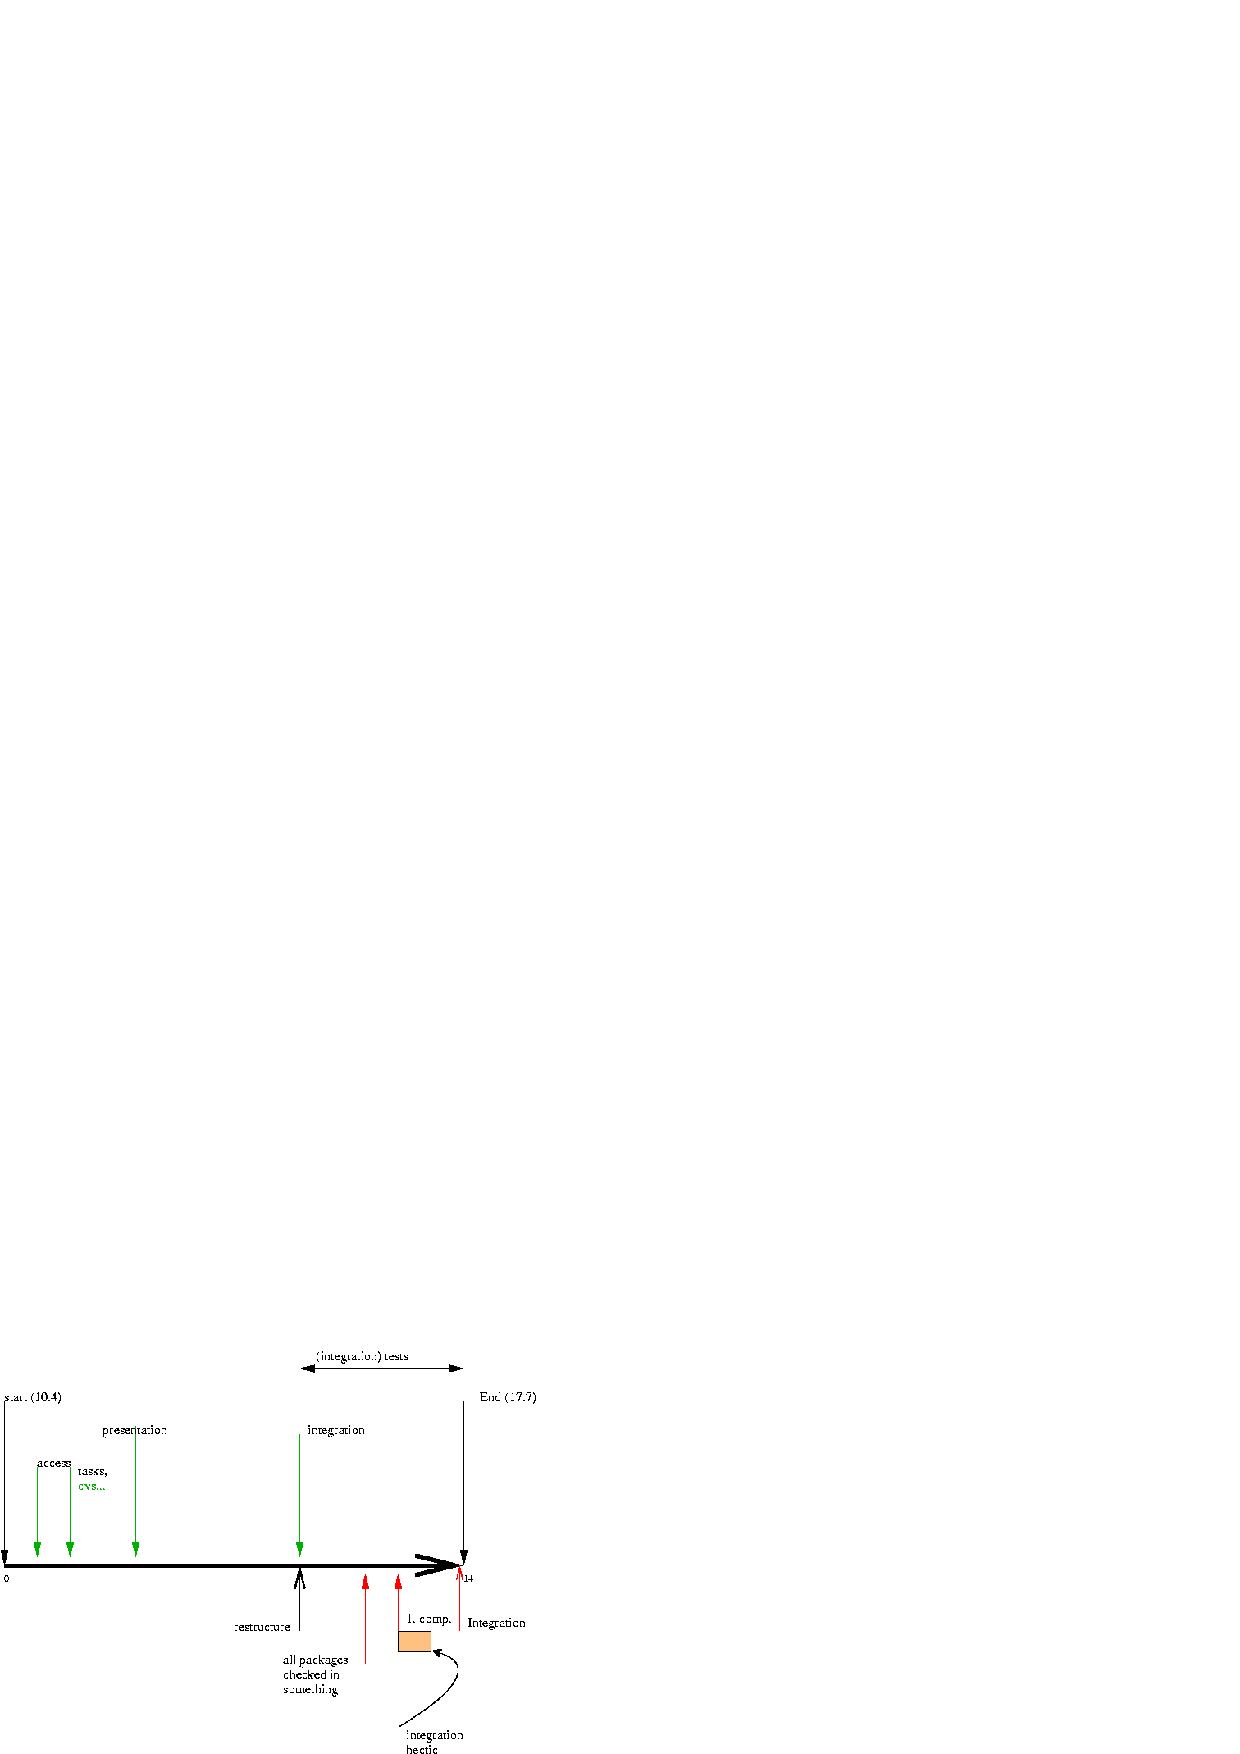
\includegraphics[height=6cm]{timeline}  
  \end{center}}







\section{Evaluation}



\frame{\frametitle{What's good?}
  \begin{itemize}
  \item<2-> it's \importantx{over}!
    \only<3->{
    \item we have running tools ready-oid and shipped
    \item not a single \important{drop-out} during semester (that was a
      \important{serious!} problem in previous F-Praktika)
    \item the \important{task} as such was ok 
    \item \important{snert} (despite it's age and performance limitations) did
      quite \important{ok}, little down-time, \important{no data loss}
    \item quite some heterogenous environment/tool sets $\Rightarrow$ lots of
      (well, practical) stuff to cope with, to find ones way }
  \end{itemize}}

\frame{\frametitle{Neutral/beyond our control}
  \begin{itemize}
  \item many participants
  \item some communication \important{overhead}: \important{Yes!} that beyond
    our control.  Even with \important{1 person} there's communication
    overhead\footnote{if the task is big enough/long enough, the programmer at
      some point during of the task has to communicate with the programmer
      later state (himself, only older), for instance via documentation.}
  \item little \important{theory} (some people like that, some don't)
    \begin{itemize}
    \item[-] in addition to (fail to) \important{work together} and
      \important{get organized} etc, we did not learn \important{anything
        theoretical}
    \item[+] more effort into other stuff.
    \end{itemize}
  \item lot's of tiny little problems: well, that how it is \ldots
  \end{itemize}
}
\frame{\frametitle{Things we did not like}
  \begin{itemize}
  \item \importantx{passivity} 
  \item some internal \importantx{in-fighting} within some groups
  \item ``\important{death march}'' or at least monstrous hectic at the end
    (year after it's the same)\footnote{Actually, it seems almost to be
      a universal constant for all human endeavor \ldots}
  \item \importantxx{laaaate} integration/testing on the target platform (year
    after year, it's the same)\footnote{In this year, it was in some of the
      groups in particular postpone \importantxx{till the veeerry end} to try
      out \emph{snert} even if it was said from the beginning: there is
      exactly/only \important{one platform} which counts, namely snert. Note
      that even if we pretended that we intend to do it platform-independent,
      announcing a predefined machine in advance is of course the opposite of
      platform-independence.}
  \item we did not manage to have a \important{common spec}
    \begin{itemize}
    \item the common \important{data model} costed to much sweat/time/friction
      already, the course was on the brink of breaking!
    \item we (as org) did not had the \important{time} to hunt after that
      issue as we tried for the data-model spec.
    \end{itemize}
  \end{itemize}
}


\frame{\frametitle{Other remarks, heard}
  \begin{itemize}
  \item the task is \importantxx{too small} for so many
    people?\footnote{remarked by more than one participant. E.g. in the form
      ``If I were alone, I could \ldots''}
    \begin{itemize}
    \item well, could indeed be\ldots \only<2->{\importantx{But think again!}
        This implies either
        \begin{itemize}
        \item only projects with \important{less people} are possible, or
        \item \importantx{adding} more requirements/tasks/feature would have
          made it \importantx{simpler!}
        \end{itemize}}
    \end{itemize}
  \item \importantxx{too many comm. channels}\ actually, we don't exactly know
    what to leave out
    \begin{itemize}
    \item indispensable: \important{svn}, also
      \important{bugzilla}\footnote{Some did not like bugzilla, but I think it was
        more important to have some bug tracking}
    \item \important{bulletin board:} you will have noticed: the BB went much
      out of use lately, when the hacking effort became harder!
    \end{itemize}
  \item \important{global meetings}:
    \begin{itemize}
    \item perhaps one should make meetings smaller, 
    \item sometimes they seem to be a \important{waste of time} for most
      participants, but no: \importantxx{I'm not talking about the data-base
        discussions!} 
    \end{itemize}
  \end{itemize}
}

\frame{\frametitle{What about the org group?}
  \begin{itemize}
  \item \importantxx{be harder/stricter} (deadlines, requirements, whatever) ??
  \item \importantxx{specify} exactly what you want, and we do it
    \begin{itemize}
    \item can be advantageous. On the other hand: the challenge here was:  we
    (the org) are the \emph{clients} we know (a bit) what we want, you have to
    find a solution
    \end{itemize}
  \item \importantxx{monitor} exactly what's going on, repair \ldots
    \begin{itemize}
    \item not really possible with $> 20$ participants
    \end{itemize}
  \item \important{repeat} the \textsl{Praktikum}
    \begin{itemize}
    \item[+] less effort for us, more time for monitoring etc
    \item[+] better feeling for the hard parts, better assistance in
      ``load-balance'' etc.
    \item[-] less ``realistic'', later your boss/manager\ldots will not
      exactly know what you are doing, there won't be ``Musterl\"osungen'' in
      your later life.
    \end{itemize}
  \end{itemize}
}

\frame{\frametitle{Things to do/org better}
  \begin{itemize}
  \item not two spec groups?
    \begin{itemize}
    \item avoids bickering/merging/friction/disappointment which spec to take
    \item[-] we cannot have all the rest as tools-groups, because the tools
      groups where wasted time
    \end{itemize}
  \item \important{testing}
    \begin{itemize}
    \item the integration/set-up for the testing \important{must} be organized
      differently, this year the set-up did not work out
    \end{itemize}
  \item \important{tools/platform choice}: 
    \begin{itemize}
    \item largely a \important{waste of time}, \important{just do
        it}/\important{document it} and that's it\footnote{In realistic
        situations, the choice of weapons and platforms is of course not a
        waste of time.  In our case, I'd say it was.}
    \end{itemize}
  \item some small stuff: 
    \begin{itemize}
    \item we \important{lost} some weeks:
      \begin{itemize}
      \item for instance after the first demo,
      \item because of protracted SQL-discussion
      \item after X-mas, delay in the status/plan 
      \end{itemize}
    \end{itemize}
  \item hard \importantxx{deadline/milestone} around X-mas
  \end{itemize}
  
}




\frame{\frametitle{Famous quotes from development hell}
  
  We collected those during this semester (sources kept
  \important{anonymous})

  \bigskip

  \only<1>{
    \shadowbox{
      \begin{minipage}[t]{11cm}
        \begin{quote}
          ``in the course of Hanus, the work-load is 3 times as hard, and
          it scores only 4 hours''
        \end{quote}
      \end{minipage}
    }}

  \only<2>{
    \shadowbox{
      \begin{minipage}[t]{11cm}
        \begin{quote}
          ``if the testers/some others needs a \texttt{Readme} to understand
          what's going on in my code, then they are free to let it
          be''\footnote{See again the foil with the ``raw and mindless
            statistic'' and think of an answer to that yourself.}
        \end{quote}
      \end{minipage}}
  }


  \only<3>{
    \shadowbox{
      \begin{minipage}[t]{11cm}
        \begin{quote}
          \emph{``of course we have a spec; it's not written down,
            however, because we have it all in our head''}\footnote{Ya, ya}
        \end{quote}
      \end{minipage}
    }}

  \only<4>{
    \shadowbox{
      \begin{minipage}[t]{11cm}
        \begin{quote}
          year after year our \emph{all-time favorite:} \textit{``it's not my
            fault. At my machine it works\ldots''}\footnote{shorter still:
            ``Ah, \important{trust me}, you don't need to try it. It works!''.
            A variant is ``we don't need to test it \important{there}, because
            it works \important{here}''. still shorter: it's
            \important{compatible}!}
        \end{quote}
      \end{minipage}
    }}

  \only<5>{
    \shadowbox{
      \begin{minipage}[t]{11cm}
        \begin{quote}
          integration will be a piece of cake, don't worry.
        \end{quote}
      \end{minipage}
    }}

  \only<6-7>{
    \shadowbox{
      \begin{minipage}[t]{11cm}
        \begin{quote}
          Request from group-X to their tester:\emph{``additionally, an
            \important{installation} test\footnote{1. February} would be
            handy, such that our tool is installed in a ``Weissbrotwelt'' as
            well''}\only<6-7>{\footnote{in the same bug thread a comment is
              again the classic: ``bei mir aufm Laptop funktioniert alles''.}}
          \only<7>{and please note down exactly what steps are needed
            [\ldots].  We have the problem that \important{we}\footnote{the
              programmers/developers!}  have forgotten what we did to install
            our tool.''\footnote{Remember the
              \textsl{``Real-programmers-don't-need-Readme's''}-comment 2
              minutes ago?}}
        \end{quote}
      \end{minipage}
    }}

}





\frame{\frametitle{Why is it not a tool?}
  \only<1>{
  \shadowbox{
    \begin{minipage}[t]{11cm}
      \begin{quote}
        The result/the process is not ``\important{professional}'', why is
        this?\footnote{Professional in the sense of ``good''
          (best-practice/state-of-the-art, or whatever jargon word you prefer).
          ``Professional'' is not meant in the sense of making a living out of it.
          After all, rather soon \important{you are professional} computer
          experts/scientists! Also it does not imply that all tools that one can
          sell/buy are better than yours \ldots }
      \end{quote}
    \end{minipage}}}

\only<2>{
  \begin{itemize}
  \item well, we listed some points which we think did not work/haven't been
    organized too well
  \item almost everyone was mainly busy with \important{his module}, little
    serious effort outside one's own home ground field.\footnote{we don't know
      directly, it's an impression: especially the PHP1 group, they kept
      problems ---if they had any--- under the carpet.}
  \item \important{symptom}: in the general meetings: desinterest or even
    \important{``bad vibes''} if ``\importantx{forced}'' to discuss things
    beyound one owns interest\footnote{Indeed, the SQL-discussion started to
      go bitter, for somehow unwillingness to take the effort. The general
      feeling was: ``C'mon, it's a waste of time, to agree on this/to discuss
      this, leave us alone.''}
  \item[$\Rightarrow$] \importantx{much more} effort into ``boring'' stuff]
    e.g., 2 persons (or more) in a group doing nothing else than
    \important{integrating,} checking whether all \important{fits together,}
    having an \important{technical overview} over the \important{interplay},
    perhaps group ``sub-leader''
    \begin{itemize}
    \item difficult in a course: ``what's my contribution?'', ``do I pass the
      exam without a line of code written?'', who is the subleader
    \end{itemize}
  \item one single semester afterwards: just
    \important{testing}/documenting/making it usable?
  \end{itemize}}
  }

\iffalse



\begin{myslide}{Results}
  \begin{itemize}
  \item runnable tool, all modules integrated, executable under jdk-1.4
    \begin{itemize}
    \item graphical interface for editing
    \item checks (type checking, well-formed checking)
    \item parser
    \item simulator
    \end{itemize}
  \item \important{CD-Rom} with jar'ed tool (+ doc + sources + repos
    \ldots)
  \end{itemize}
\end{myslide}










\begin{myslide}{Error reporting}
  \begin{lstlisting}{}
 --------------------------------------------------------
  Error <nr>:    <short description>
    package:     <in which package/class does it occur
    status:      reported|confirmed|non-confirmed|repaired
                 repaired-confirmed

               + <date> + <author>
   
    class:       fatal|non-fatal|
                 feature-request|coding convention violation ....

    description: <longer description, hints for repair>
   -----------------------------------------------------
  \end{lstlisting}
\end{myslide}



\begin{myslide}{Statistics}
  \begin{itemize}
  \item 13 official meetings
  \item 4 iterations of the requirement specification
  \item \important{> 500} emails concerning \Slime\ in my
    mailbox\footnote{including those exchanged directly with the
      participants, but without the more than 700 cvs-log emails.}
  \item approximately
    \begin{itemize}
    \item \important{100} officially reported errors\footnote{none
        confirmed \ldots}
    \item \important{170} Java files
    \item \important{200} class files, i.e. 200 public classes
    \item \important{50} \LaTeX-files (doc, web-pages, requirements)
    \item handfull of other files (Makefiles, Error lists etc.)
    \end{itemize}
  \end{itemize}
\end{myslide}






  
\end{myslide}
\begin{myslide}{Neutral/beyond our control}
  \begin{itemize}
  \item not much people, 
  \item lot of (late) drop outs,\footnote{people at the beginning:
      \important{11} (except coaches), at the end: \important{4}} and
    lately announced
  \end{itemize}
\end{myslide}

\begin{myslide}{Less good}
  \begin{itemize}
  \item \important{Attracting} students
    \begin{itemize}
    \item another topic?
    \item stressing collaborative  work over programming in \Java?
    \end{itemize}
  \item \important{laaaate} first code delivery (26.\ June) /compilation,
    \important{laaate} integration (with all the consequences)
  \item we always had quite some breaches of \important{interfaces}, but:
    this year was the first time, I had to \important{discuss} why this is
    should be avoided without much discussion
  \item communication
  \item no test group, no Error ever \texttt{confirmed}
  \end{itemize}
\end{myslide}

\begin{myslide}{Next time}
  \begin{itemize}
  \item first \emph{Readme} or first \important{written plan}
    \important{required} to be \important{checked-in} in after 2 weeks
  \item stricter, enforced cvs-strategy?: \important{enforced
    compilability} for checking-in?
\item user \important{logging} (currently, I don't know how, the official
  university's server can do it, but there are other disadvantages of that
  solution)?
  \item stricter surveillance (e.g.\ for absynt), \important{watches}
  \item no \important{separation} between gui and editor? But an explicit
    \important{test} group.
  \item other means of communication? (\emph{news-group?}, cvs-logs?)
  \end{itemize}
\end{myslide}

\fi

%%% Local Variables: 
%%% mode: latex
%%% TeX-master: "main"
%%% End: 


\bibliographystyle{alpha}
\bibliography{string,etc,crossref}

%----------------------------------------------------------------------


\end{document}

%%%%%%%%%%%%%%%%%%%%%%%%%%%%%%%%%%%%%%%%%%%%%%%%%%%%%%%%%%%%
%% $Id: main-coma.tex,v 1.3 2004/10/20 06:57:05 swprakt Exp $
%%%%%%%%%%%%%%%%%%%%%%%%%%%%%%%%%%%%%%%%%%%%%%%%%%%%%%%%%%%%
%%% Local Variables: 
%%% mode: latex
%%% TeX-master: t
%%% End: 



